% Options for packages loaded elsewhere
\PassOptionsToPackage{unicode}{hyperref}
\PassOptionsToPackage{hyphens}{url}
%
\documentclass[
  12pt,
]{article}
\usepackage{lmodern}
\usepackage{amsmath}
\usepackage{ifxetex,ifluatex}
\ifnum 0\ifxetex 1\fi\ifluatex 1\fi=0 % if pdftex
  \usepackage[T1]{fontenc}
  \usepackage[utf8]{inputenc}
  \usepackage{textcomp} % provide euro and other symbols
  \usepackage{amssymb}
\else % if luatex or xetex
  \usepackage{unicode-math}
  \defaultfontfeatures{Scale=MatchLowercase}
  \defaultfontfeatures[\rmfamily]{Ligatures=TeX,Scale=1}
\fi
% Use upquote if available, for straight quotes in verbatim environments
\IfFileExists{upquote.sty}{\usepackage{upquote}}{}
\IfFileExists{microtype.sty}{% use microtype if available
  \usepackage[]{microtype}
  \UseMicrotypeSet[protrusion]{basicmath} % disable protrusion for tt fonts
}{}
\makeatletter
\@ifundefined{KOMAClassName}{% if non-KOMA class
  \IfFileExists{parskip.sty}{%
    \usepackage{parskip}
  }{% else
    \setlength{\parindent}{0pt}
    \setlength{\parskip}{6pt plus 2pt minus 1pt}}
}{% if KOMA class
  \KOMAoptions{parskip=half}}
\makeatother
\usepackage{xcolor}
\IfFileExists{xurl.sty}{\usepackage{xurl}}{} % add URL line breaks if available
\IfFileExists{bookmark.sty}{\usepackage{bookmark}}{\usepackage{hyperref}}
\hypersetup{
  pdftitle={Authority After the Tempest: Hurricane Michael and the 2018 Elections},
  pdfauthor={Kevin Morris; Peter Miller},
  hidelinks,
  pdfcreator={LaTeX via pandoc}}
\urlstyle{same} % disable monospaced font for URLs
\usepackage[margin=1in]{geometry}
\usepackage{longtable,booktabs}
\usepackage{calc} % for calculating minipage widths
% Correct order of tables after \paragraph or \subparagraph
\usepackage{etoolbox}
\makeatletter
\patchcmd\longtable{\par}{\if@noskipsec\mbox{}\fi\par}{}{}
\makeatother
% Allow footnotes in longtable head/foot
\IfFileExists{footnotehyper.sty}{\usepackage{footnotehyper}}{\usepackage{footnote}}
\makesavenoteenv{longtable}
\usepackage{graphicx}
\makeatletter
\def\maxwidth{\ifdim\Gin@nat@width>\linewidth\linewidth\else\Gin@nat@width\fi}
\def\maxheight{\ifdim\Gin@nat@height>\textheight\textheight\else\Gin@nat@height\fi}
\makeatother
% Scale images if necessary, so that they will not overflow the page
% margins by default, and it is still possible to overwrite the defaults
% using explicit options in \includegraphics[width, height, ...]{}
\setkeys{Gin}{width=\maxwidth,height=\maxheight,keepaspectratio}
% Set default figure placement to htbp
\makeatletter
\def\fps@figure{htbp}
\makeatother
\usepackage[normalem]{ulem}
% Avoid problems with \sout in headers with hyperref
\pdfstringdefDisableCommands{\renewcommand{\sout}{}}
\setlength{\emergencystretch}{3em} % prevent overfull lines
\providecommand{\tightlist}{%
  \setlength{\itemsep}{0pt}\setlength{\parskip}{0pt}}
\setcounter{secnumdepth}{5}
\usepackage{rotating}
\usepackage{setspace}
\newcommand{\beginsupplement}{\setcounter{table}{0}  \renewcommand{\thetable}{A\arabic{table}} \setcounter{figure}{0} \renewcommand{\thefigure}{A\arabic{figure}}}
\usepackage{lineno}
\linenumbers
\usepackage{booktabs}
\usepackage{longtable}
\usepackage{array}
\usepackage{multirow}
\usepackage{wrapfig}
\usepackage{float}
\usepackage{colortbl}
\usepackage{pdflscape}
\usepackage{tabu}
\usepackage{threeparttable}
\usepackage{threeparttablex}
\usepackage[normalem]{ulem}
\usepackage{makecell}
\usepackage{xcolor}
\ifluatex
  \usepackage{selnolig}  % disable illegal ligatures
\fi
\newlength{\cslhangindent}
\setlength{\cslhangindent}{1.5em}
\newlength{\csllabelwidth}
\setlength{\csllabelwidth}{3em}
\newenvironment{CSLReferences}[2] % #1 hanging-ident, #2 entry spacing
 {% don't indent paragraphs
  \setlength{\parindent}{0pt}
  % turn on hanging indent if param 1 is 1
  \ifodd #1 \everypar{\setlength{\hangindent}{\cslhangindent}}\ignorespaces\fi
  % set entry spacing
  \ifnum #2 > 0
  \setlength{\parskip}{#2\baselineskip}
  \fi
 }%
 {}
\usepackage{calc}
\newcommand{\CSLBlock}[1]{#1\hfill\break}
\newcommand{\CSLLeftMargin}[1]{\parbox[t]{\csllabelwidth}{#1}}
\newcommand{\CSLRightInline}[1]{\parbox[t]{\linewidth - \csllabelwidth}{#1}\break}
\newcommand{\CSLIndent}[1]{\hspace{\cslhangindent}#1}

\title{Authority After the Tempest: Hurricane Michael and the 2018 Elections}
\author{Kevin Morris\footnote{Researcher, Brennan Center for Justice at NYU School of Law, 120 Broadway Ste 1750, New York, NY 10271 (\href{mailto:kevin.morris@nyu.edu}{\nolinkurl{kevin.morris@nyu.edu}})} \and Peter Miller\footnote{Researcher, Brennan Center for Justice at NYU School of Law, 120 Broadway Ste 1750, New York, NY 10271 (\href{mailto:peter.miller@nyu.edu}{\nolinkurl{peter.miller@nyu.edu}})}}
\date{May 21, 2021}

\begin{document}
\maketitle
\begin{abstract}
Hurricane Michael made landfall in the Florida panhandle 27 days before the 2018 elections. In the aftermath, the governor of Florida issued Executive Order 18-283 granting election officials in 8 impacted counties the autonomy to loosen a variety of voting laws related to early in-person voting, voting by mail ballots, and the number and location of polling places to ensure the orderly conduct of the election. To test the efficacy of the order we deploy a novel research design to separate the effects of the hurricane on turnout from the administrative effects of actions taken by election officials. By leveraging cross-jurisdiction variation in a double-matched, triple-differences model, we show that the executive order was not successful at eliminating declining turnout. As administrators loosen mail-voting restrictions in advance of this fall, they must couple these eased restrictions with strong public education campaigns about how voters can take advantage of them. \textbf{Do we need to revise the abstract in light of new results?}
\end{abstract}

\pagenumbering{gobble}
\pagebreak

\pagenumbering{arabic}
\doublespacing

\hypertarget{introduction}{%
\section*{Introduction}\label{introduction}}
\addcontentsline{toc}{section}{Introduction}

As the 2018 elections approached, an unanticipated -- but not unprecedented -- shape appeared on the Florida horizon: the Category 5 Hurricane Michael.\footnote{The category of the hurricane refers to the maximum sustained wind speed, according to the Saffir-Simpson hurricane wind scale. A Category 5 hurricane sustains winds greater than 157 miles per hour, \textbf{as measured as the peak 1-minute wind at a height of 33 feet. See \url{https://www.nhc.noaa.gov/pdf/sshws.pdf}.}} The hurricane made landfall on October 10, 27 days before the election, and would ultimately cause 16 deaths and 25 billion dollars in damage.\footnote{See \url{https://www.nhc.noaa.gov/data/tcr/AL142018_Michael.pdf}.} Would-be voters in the election were now faced with myriad disruptions to their daily lives; the direct effects of the weather, therefore, likely reduced turnout substantially as the recovery from the hurricane progressed. As professor emeritus Robert Montjoy told NPR in the aftermath of the storm, ``Whether casting a ballot becomes a higher priority than cleaning out the basement, visiting someone in the hospital, or all the other demands\ldots You certainly expect a lower turnout for those reasons'' (\protect\hyperlink{ref-Parks2018}{Parks 2018}).

The storm also affected the administration of the election itself, as polling places were destroyed and potential mail voters found themselves temporarily residing at addresses other than those at which they were registered. The governor of Florida issued Executive Order 18-283\footnote{See \url{https://www.flgov.com/wp-content/uploads/2018/10/SLT-BIZHUB18101809500.pdf}.} as a means to counteract the widespread effects of the hurricane on October 18. Executive Order 18-283 sought to offset the administrative barriers to voting by allowing election administrators in 8 counties in Florida affected by the hurricane to flexibly respond to the damage wrought by the storm. Specifically, Executive Order 18-283 allowed administrators to add early voting locations; begin early voting 15 days before the general election (4 days after the Executive Order was issued), and continue until the day of the election; to accept vote-by-mail requests to addresses other than a voter's registered address; to send vote-by-mail ballots by forwardable mail; to deliver vote-by-mail ballots to electors or electors' immediate family members on election day without an affidavit; to relocate or consolidate polling places; and required poll watchers to be registered by the second Friday before the general election. The executive order covered Bay, Calhoun, Franklin, Gadsden, Gulf, Jackson, Liberty, and Washington Counties.

This paper sets out to answer a number of questions: what was the total depressive effect of the hurricane? Did Executive Order 18-283 effectively offset the depressive administrative effects? More specifically, did easing mail-balloting and early voting rules reduce the impact of closed polling places? We propose a novel research design to investigate these interrelated questions -- what we are calling a double-matched, triple-difference model -- and then demonstrate that the hurricane significantly reduced turnout and that responses to the hurricane by local election officials were unable to overcome the devastation of the hurricane. We conclude with some thoughts about how the instance of Hurricane Michael can inform the conduct of elections under other natural disasters \textbf{likely to occur in the future}\sout{the COVID-19 pandemic (\protect\hyperlink{ref-James2020}{James and Alihodzic 2020})}.

\hypertarget{literature-review}{%
\section*{Literature Review}\label{literature-review}}
\addcontentsline{toc}{section}{Literature Review}

This study lies at the intersection of three components of the broader turnout literature: the effects of inclement and severe weather, the capacity for convenience voting reforms to increase participation in elections, and the ability of local election officials to increase turnout by placing polls where voters are able to access them. Our general observation is that while the effects of weather are often negative with regard to participation in elections, the leverage for voting reforms and local officials to counterbalance those depressive effects are limited.

\hypertarget{weather-effects}{%
\subsection*{Weather Effects}\label{weather-effects}}
\addcontentsline{toc}{subsection}{Weather Effects}

\textbf{Variations in weather on election day are generally thought be exogenous to elections (\protect\hyperlink{ref-Cooperman2017}{Cooperman 2017}; \protect\hyperlink{ref-Hansford2010}{Hansford and Gomez 2010, 269}), but also have an effect on turnout. \protect\hyperlink{ref-Rallings2003}{Rallings, Thrasher, and Borisyuk} (\protect\hyperlink{ref-Rallings2003}{2003}) observes ``{[}v{]}ariable weather patterns are also likely to affect turnout since these too would be regarded as a variable cost in the act of voting'' (78). Rainfall in Irish parliamentary elections, for one recent example of a larger comparative literature, reduces turnout, especially in densely populated districts (\protect\hyperlink{ref-Garcia-Rodriguez2020}{\textbf{Garcia-Rodriguez2020?}}). However, a study in Sweden (\protect\hyperlink{ref-Persson2014}{Persson, Sundell, and Öhrvall 2014}) found no significant turnout effects of rain on election day in part due to Sweden's permissive early voting regime; voters were able to avoid an incoming storm by casting a ballot in advance. Furthermore, and most relevant to our study of Hurricane Michael, is the effect of Typhoon Lan\footnote{Lan was the equivalent of a Category 4 hurricane, featuring wind speeds of between 130 and 156 miles per hour.} on turnout in the 2017 House of Representatives election in Japan. The typhoon made landfall the day after election day, though it appears voters behaved dynamically as the typhoon approached: voters were more likely to vote early, or earlier on the day of the election, as rainfall increased in prefectures in the path of the typhoon (\protect\hyperlink{ref-Kitamura2020}{Kitamura and Matsubayashi 2020}). Our study of Hurricane Michael informs both American and comparative experience with holding an election in the face of inclement and sometimes severe weather.}

This question has \textbf{also} been frequently examined in the United States. While the studies produce divergent point estimates, the consensus is that turnout is lower in the presence of rain on election day (\protect\hyperlink{ref-Cooperman2017}{Cooperman 2017}; \protect\hyperlink{ref-Fujiwara2016}{Fujiwara, Meng, and Vogl 2016}; \protect\hyperlink{ref-Hansford2010}{Hansford and Gomez 2010}; \protect\hyperlink{ref-Fraga2010}{Fraga and Hersh 2010}; \protect\hyperlink{ref-Gomez2007}{Gomez, Hansford, and Krause 2007}; \protect\hyperlink{ref-Shachar1999}{Shachar and Nalebuff 1999}; \protect\hyperlink{ref-Knack1994}{Knack 1994}; \protect\hyperlink{ref-Merrifield1993}{Merrifield 1993}). The effect of rain on turnout, however, is strongest among voters with less of a sense that voting is a civic duty and altogether absent among voters with a strong sense of civic duty (\protect\hyperlink{ref-Knack1994}{Knack 1994}). \protect\hyperlink{ref-Fraga2010}{Fraga and Hersh} (\protect\hyperlink{ref-Fraga2010}{2010}) find the decrease in turnout is only found in noncompetitive counties; a competitive race is sufficient to induce voters to cast a ballot in the rain. \protect\hyperlink{ref-Gatrell2002}{Gatrell and Bierly} (\protect\hyperlink{ref-Gatrell2002}{2002}) find the effect of rain is most pronounced in general elections (where more peripheral voters are brought into the electorate) than primary elections (where the electorate tends to be more partisan).

Rain on election day may not be relevant to the considerably more severe damage that follows after a hurricane. Previous natural disasters, such as Hurricane Sandy (2012) in Connecticut, New Jersey and New York and Hurricane Katrina (2005) in New Orleans, may give a better set of boundary conditions on our expectations of how severe, as opposed to inclement, weather may alter electoral behavior. Studies of these events found lower turnout within effected geographic areas (\protect\hyperlink{ref-Lasala-Blanco2017}{Lasala-Blanco, Shapiro, and Rivera-Burgos 2017}; \protect\hyperlink{ref-Stein2015}{Stein 2015}; \protect\hyperlink{ref-Debbage2014}{Debbage et al. 2014}; \protect\hyperlink{ref-Sinclair2011}{Sinclair, Hall, and Alvarez 2011}). \protect\hyperlink{ref-Sinclair2011}{Sinclair, Hall, and Alvarez} (\protect\hyperlink{ref-Sinclair2011}{2011}) also find non-linear effects, where people who experienced considerable flooding were \emph{more} likely to vote in the subsequent election. One factor to bear in mind, however, is the timing of these storms relative to an election. Hurricane Sandy (a Category 3 hurricane) made landfall eight days before the 2012 elections; Katrina (Category 5) made landfall more than a year before the 2006 elections. Hurricane Michael (Category 5) made landfall 27 days before the 2018 elections. We expect, therefore, that the effects of Michael with regard to turnout may be closer in magnitude to the effects observed in the aftermath of Sandy rather than Katrina, despite Michael and Katrina being of comparable wind speed upon landfall.

\hypertarget{early-voting-and-turnout}{%
\subsection*{Early voting and turnout}\label{early-voting-and-turnout}}
\addcontentsline{toc}{subsection}{Early voting and turnout}

Florida, like Sweden, has a permissive convenience voting regime (\protect\hyperlink{ref-Gronke2008}{Gronke et al. 2008}). Registered voters can present themselves at an early in-person polling place to cast a ballot in advance of election day. Registered voters can also request a mail ballot on an unrestricted basis and return that ballot before the election. Can these reforms increase turnout? This question is not yet resolved in the literature; we are left unsatisfyingly answering the question about turnout effects of convenience voting reforms with both ``\,`no' and `yes'\,'' (\protect\hyperlink{ref-Bergman2015}{Bergman 2015}).

There is evidence for a variety of effects when looking at turnout effects of convenience voting reforms. Early in-person voting increased turnout in the 1994 elections among Tennessee counties (\protect\hyperlink{ref-Ricardson1996}{Ricardson and Neeley 1996}). A study from Ohio found an additional day of early in-person voting increased turnout (\protect\hyperlink{ref-Kaplan2020}{Kaplan and Yuan 2020}). That being said, early voting \emph{decreased} turnout in the 2000, 2004, and 2008 elections (\protect\hyperlink{ref-Larocca2011}{Larocca and Klemanski 2011}; \protect\hyperlink{ref-Burden2014}{Burden et al. 2014}). \sout{The literature on turnout effects of elections conducted entirely via the mail, however, is similarly mixed.} \textbf{Studies of recent elections find absentee voting increases turnout (\protect\hyperlink{ref-Leighley2014}{Leighley and Nagler 2014}; \protect\hyperlink{ref-Larocca2011}{Larocca and Klemanski 2011}), though that effect is not found in elections between 1972 and 2002 (\protect\hyperlink{ref-Fitzgerald2005}{Fitzgerald 2005})}. \sout{The picture is no clearer when we look at elections conducted entirely by mail. That reform increases turnout in Washington (\protect\hyperlink{ref-Henrickson2019}{Henrickson and Johnson 2019}; \protect\hyperlink{ref-Gerber2013}{Gerber, Huber, and Hill 2013}), decreases turnout in California (\protect\hyperlink{ref-Elul2017}{Elul, Freeder, and Grumbach 2017}; \protect\hyperlink{ref-Bergman2011}{Bergman and Yates 2011}; \protect\hyperlink{ref-Kousser2007}{Kousser and Mullin 2007}), and has no significant effect in Oregon (\protect\hyperlink{ref-Gronke2012}{Gronke and Miller 2012}). A recent, national study finds a small boost to turnout following from the adoption of Oregon-style voting by mail (\protect\hyperlink{ref-Barber2020}{Barber and Holbein 2020}).}

\hypertarget{polling-place-consolidation}{%
\subsection*{Polling Place Consolidation}\label{polling-place-consolidation}}
\addcontentsline{toc}{subsection}{Polling Place Consolidation}

One element of election administration that local authorities can control is the location of polling places. Relocating or reducing the number of polling places in turn reduces turnout by imposing new search and transportation costs on voters (\protect\hyperlink{ref-Brady2011}{Brady and McNulty 2011}). A moved polling place reduces turnout in a variety of electoral contexts (\protect\hyperlink{ref-Cantoni2020}{Cantoni 2020}), including local elections (\protect\hyperlink{ref-McNulty2009}{McNulty, Dowling, and Ariotti 2009}; \protect\hyperlink{ref-Haspel2005}{Haspel and Knotts 2005}) as well as national contests (\protect\hyperlink{ref-Kropf2012}{Kropf and Kimball 2012}). Absentee voting is more likely as the distance to the polls increases, but this effect is not large enough to offset the decrease from consolidation itself (\protect\hyperlink{ref-Brady2011}{Brady and McNulty 2011}; \protect\hyperlink{ref-Dyck2005}{Dyck and Gimpel 2005}).

The effect of distance to the polling place on voting is nonlinear (\protect\hyperlink{ref-Dyck2005}{Dyck and Gimpel 2005, 541--42}; \protect\hyperlink{ref-Gimpel2003}{Gimpel and Schuknecht 2003, 481--84}). A study of three counties in Maryland in the 2000 election finds moving 1 mile \emph{closer} to the polls makes voting \emph{more} likely by 0.45 points, while observing generally ``{[}t{]}urnout is highest when distances to the polling place are very short, and when they are excessively long, but lower in the middling ranges of distance'' (\protect\hyperlink{ref-Gimpel2003}{Gimpel and Schuknecht 2003, 481}).

\textbf{We probably want to say more about how polling place consolidation informs our paper, in light of another of R1's comments, and I thought the best place for that would be a new paragraph here}

\textbf{The executive order issued after Hurricane Michael empowered local election officials in the eight affected counties with the autonomy to move or consolidate polling places at will. According to public records we obtained, these counties collectively saw about half of the anticipated (62 of the 127) polling places opened in the election.}

\textbf{Here is where I try to explain how we think the effect of a hurricane is conditional on election adminstration, but only based on one study}

\textbf{We know remarkably little about the interactive or conditional effects early voting, severe weather, and polling place consolidation have on turnout. The only paper we know of that explores the conditional effect of early voting in the context of a natural disaster is Stein's study of Hurricane Sandy (\protect\hyperlink{ref-Stein2015}{Stein 2015}). Stein observes that residing in a county that was covered by the disaster and provided for early in-person voting exhibited \emph{increased} turnout in 2012. We know of no studies that examine the effect of no-excuse absentee voting on turnout in the aftermath of a natural disaster, the causal relationship between early voting and polling place consolidation, or the effect of rain or other weather on the availability or accessibility of polling places.}

Grounding our analyses of the effects of Hurricane Michael gives us some expectations as to how the hurricane will alter voting behavior. We expect the direct, weather-related effects of the hurricane to reduce turnout. The administrative effects will push in operate directions. On the one hand, consolidated polling places likely imposed costs on voters, reducing turnout above-and-beyond on the individual effects. On the other hand, the loosened restrictions on mail voting and relief valve offered by early voting may recover \emph{some but not all} of these displaced voters. This is, of course, not to claim that the local officials in the path of the hurricane sought to reduce turnout. Rather, the work of administering an election --- even under the best of circumstances --- is difficult. The extraordinary impact of a Category 5 hurricane is perhaps simply too much for election administrators to incorporate into their efforts to conduct a secure and inclusive election.

\hypertarget{research-design-and-expectations}{%
\section*{Research Design and Expectations}\label{research-design-and-expectations}}
\addcontentsline{toc}{section}{Research Design and Expectations}

We expect that Hurricane Michael depressed turnout in the 2018 midterm election via two causal mechanisms: individual-level effects, and administrative effects. Throughout our analyses, we examine the effect of the hurricane on voters registered as of the 2018 election. Put differently, we do not test the turnout of \emph{eligible citizens}. Conditioning turnout on registration status raises important questions when the treatment might influence registration (see \protect\hyperlink{ref-Nyhan2017}{Nyhan, Skovron, and Titiunik 2017}). That is likely the case here: as we demonstrate in the Supplemental Information, it seems probable that Hurricane Michael reduced registrations in the days before the registration deadline. Our models cannot capture these turnout effects; as such, our estimated negative treatment effects should be considered conservative, as we are not measuring the turnout of individuals whose registration---and subsequent participation---was impeded by the storm.

\hypertarget{estimating-the-net-effects-of-the-hurricane}{%
\subsection*{Estimating the Net Effects of the Hurricane}\label{estimating-the-net-effects-of-the-hurricane}}
\addcontentsline{toc}{subsection}{Estimating the Net Effects of the Hurricane}

We begin by testing the net effect of each of these treatments on individual-level turnout. Our central identification strategy involves the use of difference-in-differences models. We use voter-file data from L2 Political to estimate individual-level turnout and to control for individual-level characteristics and the latitude and longitude of each voter's residential address. L2 uses models to predict individual race / ethnicity and voters' sex but these characteristics are available in self-reported form in the raw voter-file available from the state; as such, we pull sex and race / ethnicity from the publicly available voter file. The L2 data is based on the February 8, 2019, version of the raw voter file, the same file from which we pull race / ethnicity and sex.

In addition to the individual-level characteristics from the voter file, we also proxy each voter's exposure to Hurricane Michael using rainfall data. The National Oceanic and Atmospheric Administration (NOAA) makes daily rainfall data available for some 13,000 stations around the United States. At each weather station, we measure the amount of rain that fell between October 10 and November 6 in 2018 relative to the average rainfall in that period from 2000 to 2017. Voters' individual exposure to rainfall is calculated as the average of the three closest weather stations, inversely weighted by distance.

Finally, we incorporate information garnered from public records requests sent to each of the 8 treated counties about the number of polling places they closed due to Hurricane Michael. Three counties (Calhoun, Gadsden, and Liberty) closed no polling places, while a fourth (Franklin) actually added added an additional polling place. The other four covered counties cut the number of polling places by at least two-thirds. We expect the turnout effect of the storm was lower (that is, less negative) in the counties where more polling places were open.

By comparing historical and 2018 turnout for voters in the counties hit by the storm to historical and 2018 turnout of voters elsewhere in the state, we can estimate the effect of the storm on turnout. To ensure a high-quality difference-in-differences specification, we do not include all untreated voters in our control group; rather, we genetically match (\protect\hyperlink{ref-Sekhon2011}{Sekhon 2011}) each treated voter with five untreated voters along a battery of individual- and neighborhood-level characteristics, including past turnout and vote mode. Untreated voters who do not serve as matches are excluded from our models. Although it may seem counterintuitive to exclude data from our models, this matching procedure substantially improves the parallel trends assumptions necessary for a rigorous difference-in-differences analysis (\protect\hyperlink{ref-Sekhon2009}{Sekhon 2009, 496}). As we show in the Supplemental Information, our results are robust to multiple different matching approaches, as well as when we use entropy balancing.

This design allows us to test our first hypothesis:

\textbf{Hypothesis 1:} Turnout among voters in the eight treated counties was depressed in the 2018 election relative to voters in untreated counties. This represents the net effect of both the individual and administrative level treatments. We expect that these negative treatment effects will be larger in counties that closed more polling places in response to the executive order, and where the relative rainfall was higher.

\hypertarget{decomposing-individual-and-administrative-effects}{%
\subsection*{Decomposing Individual and Administrative Effects}\label{decomposing-individual-and-administrative-effects}}
\addcontentsline{toc}{subsection}{Decomposing Individual and Administrative Effects}

To estimate the administrative effect on turnout, we must control for the individual-level effects of the storm. To do so, we leverage the somewhat arbitrary borders of counties in the Florida Panhandle, an approach similar to that adopted in a different context by \protect\hyperlink{ref-Walker2019}{Walker, Herron, and Smith} (\protect\hyperlink{ref-Walker2019}{2019}). There is no reason to believe that the effects of a hurricane would change dramatically along county borders. We assume, therefore, that voters who lived nearby one another, but on either side of a county border, faced the same weather issues during the 2018 election. Within a narrow buffer around the county border, we can therefore conceive of a voter's county as effectively randomly assigned. Any observed turnout differential, therefore, is attributable to the county in which they happen to live. Our treated voters lived in counties where polling places could be closed or moved shortly before the election, and also where some restrictions were eased, which could have altered turnout.

Of course, self-selection around a geographic boundary is entirely possible; as such, conceiving of the administrative boundary as a quasi-random assignment is perhaps too strong of an assumption. Treated and control voters, despite living very near to one another, might differ in meaningful ways. To address this potential problem, we adopt the technique developed by \protect\hyperlink{ref-Keele2015a}{Keele, Titiunik, and Zubizarreta} (\protect\hyperlink{ref-Keele2015a}{2015}) by also matching voters on either side of the boundary according to their historical turnout and vote mode. To strengthen the plausibility of the assumption that treated and primary control voters faced identical storm-related effects, we also match on each voter's relative rainfall.

By comparing the 2018 turnout of these treated and control voters, we can identify the administrative effect of the hurricane on turnout for the treated voters living within the buffer around the border. By further comparing the turnout of these control voters to (matched) voters elsewhere in the state, we can also estimate the individual effects of the storm, again just for the voters who live near the administrative boundary. We call this a double-matched triple-differences (or difference-in-difference-in-differences) specification. We lay out the specific steps below.

We begin by constructing our set of treated voters. These treated voters include all registered voters who live in a treated county and within 2.5 miles of a bordering, untreated county (See Figure \ref{fig:map}). Each treated voter is then matched to one voter who lives in an untreated county, but within 2.5 miles of a treated county. These matches are considered primary control voters. Although Calhoun, Franklin, and Gulf Counties were covered by the executive order, no voters in these counties live within 2.5 miles of an untreated county; as such, these treated voters are not included in these models.

\begin{figure}[h]

{\centering 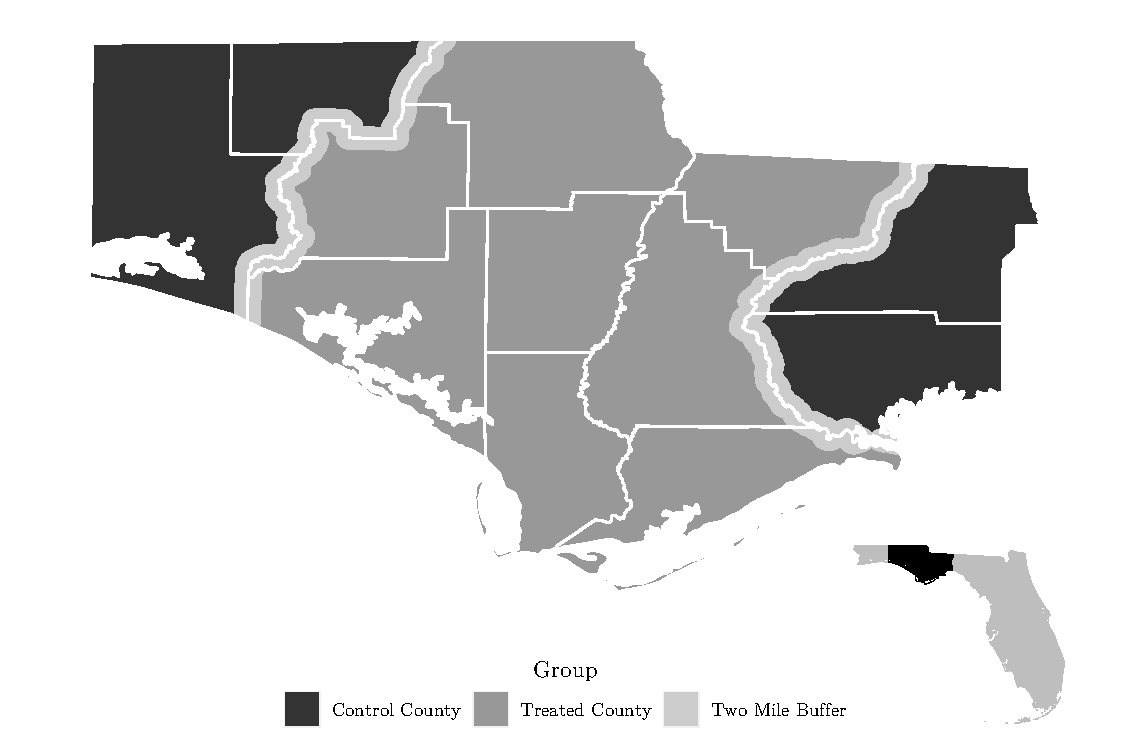
\includegraphics{hurricane_michael_files/figure-latex/map-chunk-1} 

}

\caption{\label{fig:map}Treated and Control Counties with 2.5 Mile Buffer}\label{fig:map-chunk}
\end{figure}

Each treated and primary control voter is subsequently matched to five voters elsewhere in the state --- that is to say, voters who are neither in the treated counties nor in the counties directly surrounding the treated counties. This exercise is the second match, and the matches are our ``secondary control voters.'' These voters were subject to neither individual-level nor administrative-level treatments.

At this point, we have three distinct groups of voters:

\begin{itemize}
\tightlist
\item
  Treated voters. These voters were subject to individual- and administrative-level effects from Hurricane Michael
\item
  Primary control voters. These voters were subject to individual, but not administrative, effects from Hurricane Michael.
\item
  Secondary control voters. These voters were subject to neither individual nor administrative effects.
\end{itemize}

Having constructed our pool of voters, we run a triple-differences model. This triple-differences model is, in effect, two simultaneous difference-in-differences models. The model estimates whether 2018 was associated with depressed turnout for our primary control voters vis-à-vis their controls. Because these primary control voters lived in counties not covered by the executive order, we assume that they faced no administrative effects from the storm. Any observed difference between these groups is therefore the individual-level effect of the storm for primary control voters --- and, by extension, the treated voters.

The model also estimates turnout differences between treated and primary control voters. Because we assume these closely-located voters faced identical individual-level effects, any difference between treated and primary control voters is the administrative effect on turnout of living in a treated county.

The double-matched triple-differences model allows us to test our second and third hypotheses:

\textbf{Hypothesis 2:} We expect that the hurricane had negative individual-level effects for voters who lived just outside of treated counties.

\textbf{Hypothesis 3:} We expect that the administrative effect will be largely driven by the number of polling places each county consolidated, other things equal. Where many polling places were closed we anticipate a large, negative treatment effect. In contrast, where most polling places remained open, we expect small negative or small positive administrative treatment effects.

*Here I work in the Milwaukee piece to give some support to our expectation stated in Hypothesis 3**

\textbf{A recent study of polling place consolidation in Milwaukee in light of the COVID pandemic of 2020 (\protect\hyperlink{ref-Morris2020}{\textbf{Morris2020?}}) found a significant negative effect in the city of Milwaukee compared to surrounding counties that did not experience as drastic of a consolidation.}

\hypertarget{vote-mode}{%
\subsection*{Vote Mode}\label{vote-mode}}
\addcontentsline{toc}{subsection}{Vote Mode}

After estimating the double-matched triple-differences model, we turn to vote-mode within the treated counties. We submitted public records requests to each of the eight counties covered by the executive order requesting the planned and actual location of each polling place. The changes in polling places are summarized in Table \ref{tab:moved-pps}.

To test whether the executive order shifted vote mode from in-person to mail voting in the treated counties, we begin by calculating how far each voter lived from the closest planned polling place, and how far she lived from the closest polling place that was actually open on election day. Using the registered voter file, we can tell not only \emph{whether} a voter participated, but also \emph{how} they participated. Using a multinomial logistic regression, we test whether the difference between the planned and actual distance-to-polling-place were associated with vote-mode in 2018. This specification allows us to test our final hypothesis:

\textbf{Hypothesis 4}: As the difference between the actual and planned distance to the closest polling place increased for voters, they were more likely to vote absentee and to abstain from voting, all else being held equal.

\hypertarget{results}{%
\section*{Results}\label{results}}
\addcontentsline{toc}{section}{Results}

\hypertarget{overall-turnout-effects}{%
\subsection*{Overall Turnout Effects}\label{overall-turnout-effects}}
\addcontentsline{toc}{subsection}{Overall Turnout Effects}

We begin by matching each registered voter in the eight treated counties to five untreated voters elsewhere in the state using a nearest neighbor approach. We use a genetic algorithm to determine the weight each characteristic should receive for the matching procedure (\protect\hyperlink{ref-Sekhon2011}{Sekhon 2011}).\footnote{Due to computing constraints, the matching weights were constructed using a one percent random sample stratified by treatment status. The weights derived from the genetic algorithm are then used to perform the nearest-neighbor match for all treated voters.} The individual-level characteristics come directly from the L2 and the registered voter file. The two neighborhood-level characteristics included --- median income and share of the population with some collegiate education --- are estimated at the block group level, and come from the ACS 5-year estimates ending with 2018. Ties are not broken, which means that some treated voters are assigned more than five control voters; the weights used in the regressions below are adjusted accordingly.

Although the treated counties were at the center of the storm, nearby counties might have also been negatively impacted by the storm. Therefore, voters who live in the counties that border the treated counties are excluded as potential controls. These include Walton, Holmes, Wakulla, and Leon Counties. According to public records requests we filed, none of these counties reduced polling places or early voting days because of the hurricane.

Table \ref{tab:full-bal} demonstrates the results of this matching procedure. As Table \ref{tab:full-bal} makes clear, voters in the affected counties were considerably more likely to be white and identify as Republicans, and live in lower-income neighborhoods, than voters in the rest of the state. The post-match control group, however, looks substantially similar to the treated voters.

\begin{singlespace}
\begin{table}[!h]

\caption{\label{tab:balance-tab-full}\label{tab:full-bal} Balance Table for Statewide Matching}
\centering
\resizebox{\linewidth}{!}{
\begin{tabular}[t]{lllllrrrr}
\toprule
\multicolumn{1}{c}{ } & \multicolumn{2}{c}{Means: Unmatched Data} & \multicolumn{2}{c}{Means: Matched Data} & \multicolumn{4}{c}{Percent Improvement} \\
\cmidrule(l{3pt}r{3pt}){2-3} \cmidrule(l{3pt}r{3pt}){4-5} \cmidrule(l{3pt}r{3pt}){6-9}
 & Treated & Control & Treated & Control & Mean Diff & eQQ Med & eQQ Mean & eQQ Max\\
\midrule
\%White & 76.5\% & 62.3\% & 76.5\% & 76.5\% & 100.00 & 100.00 & 100.00 & 100.00\\
\% Black & 17.1\% & 13.1\% & 17.1\% & 17.1\% & 100.00 & 100.00 & 100.00 & 100.00\\
\% Latino & 2.1\% & 17.4\% & 2.1\% & 2.1\% & 100.00 & 100.00 & 100.00 & 100.00\\
\% Asian & 1.0\% & 2.0\% & 1.0\% & 1.0\% & 100.00 & 100.00 & 100.00 & 100.00\\
\% Female & 52.5\% & 52.4\% & 52.5\% & 52.5\% & 100.00 & 100.00 & 100.00 & 100.00\\
\% Male & 45.8\% & 44.9\% & 45.8\% & 45.8\% & 100.00 & 100.00 & 100.00 & 100.00\\
Age & 52.2 & 52.5 & 52.2 & 52.2 & 98.54 & 96.68 & 97.36 & 96.17\\
\% Democrat & 39.2\% & 37.1\% & 39.2\% & 39.2\% & 100.00 & 100.00 & 100.00 & 100.00\\
\% Republican & 43.6\% & 35.0\% & 43.6\% & 43.6\% & 100.00 & 100.00 & 100.00 & 100.00\\
\% with Some College & 69.0\% & 75.1\% & 69.0\% & 69.0\% & 99.77 & 99.00 & 98.05 & 88.66\\
Median Income & \$50,643 & \$62,941 & \$50,643 & \$50,654 & 99.91 & 98.11 & 96.89 & 86.56\\
\bottomrule
\end{tabular}}
\end{table}
\end{singlespace}

Figure \ref{fig:full-to} plots the turnout in the past few elections for our treated and control voters. The left-hand panel shows the turnout of all voters. In the right-hand panel, we plot the turnout of treated voters and only their controls. As Figure \ref{fig:full-to} makes clear, turnout in the treated counties was consistently higher than the rest of the state---until 2018, when the hurricane hit. In the right-hand panel, we see that the matching procedure was successful at reducing historical differences between treated and control voters, and that there was a substantial, negative treatment effect in 2018.

\begin{figure}[h]

{\centering 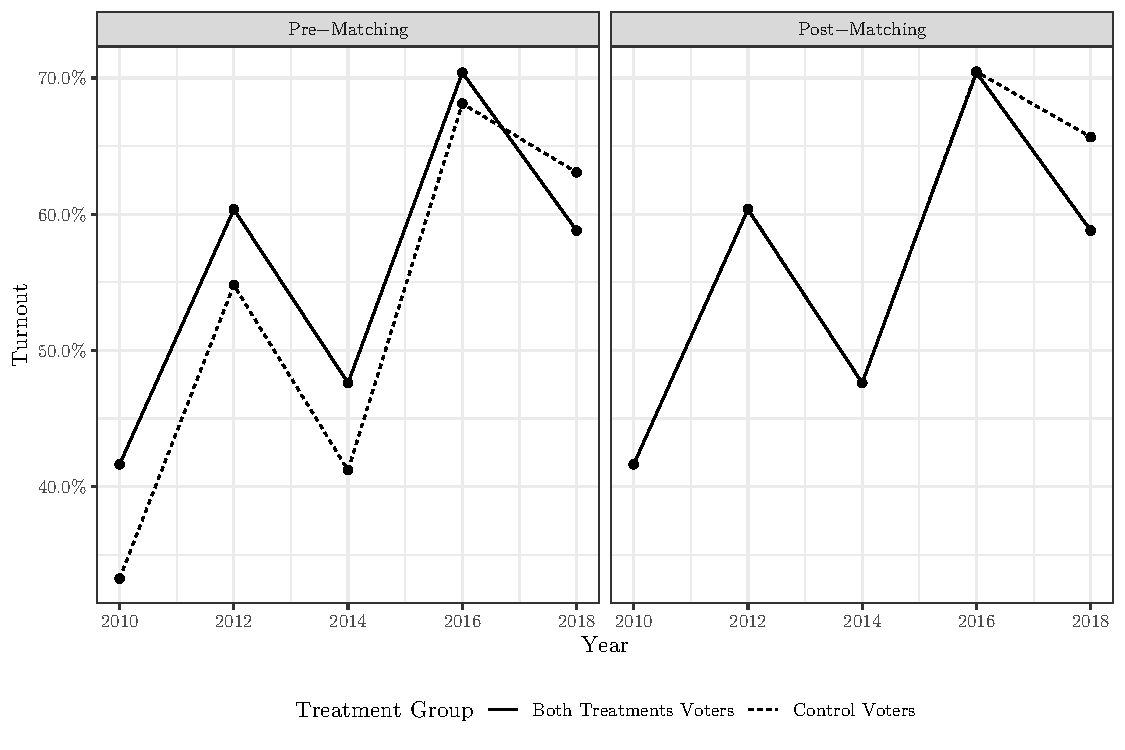
\includegraphics{hurricane_michael_files/figure-latex/full-to-chunk-1} 

}

\caption{\label{fig:full-to}General Election Turnout for Treated and Control Voters, 2010 -- 2018}\label{fig:full-to-chunk}
\end{figure}

Table \ref{tab:full-dind} formalizes the right-hand panel of Figure \ref{fig:full-to} into a differences-in-differences regression. We employ an ordinary least squares specification. The dependent variable takes the value 1 if a voter cast a ballot in a given year, and 0 if she did not. In each model, \emph{Treated × 2018} estimates the casual (net) effect of Hurricane Michael on turnout for treated voters. Model 2 also includes the characteristics on which the voters were matched. Model 3, finally, adds a measure for congressional district competitiveness. Because this variable is ``downstream'' of treatment --- that is to say, the effect of the hurricane could have impacted the competitiveness of certain races --- it is not included in the first two models. It should be noted that each of the treated voters lived in uncontested congressional districts.

In model 4, we allow for the possibility that the treatment effect was different where the hurricane had greater intensity. In this model, \emph{Treated × 2018 × Relative Rainfall} allows the treatment effect to vary based on our proxy for hurricane strength. Finally, in model 5, we ask whether the treatment effect is different in counties where fewer polling places occurred (\emph{Treated × 2018 × Share of Expected Polling Places Open}). Model 5 includes controls for hurricane strength to tease apart the effect of polling place closures from hurricane strength. Models 4 and 5, control voters are assigned the value of their treated voter. While the regressions include the full set of uninteracted and interaction terms, we display only these variables' impact on the treatment estimate in table. In each model, robust standard errors are clustered at the level of the match (\protect\hyperlink{ref-Abadie2020}{Abadie and Spiess 2020}).

\begin{singlespace}
\input{"../temp/dind_full.tex"}
\end{singlespace}

The coefficient on \emph{Treated × 2018} in Table \ref{tab:full-dind} indicates that Hurricane Michael had a substantial depressive effect in 2018 among the treated voters. Models 1 -- 3 indicate that the hurricane reduced turnout in the treated counties by roughly 6.6 percentage points. Multiplied across the nearly 200 thousand registered voters in the treated counties indicates that some 13 thousand ballots went uncast due to the hurricane, a major effect in a year when a statewide senate race was decided by 10,033 votes.

Model 4 demonstrates that the turnout effect was not moderated by the strength of the hurricane. It should be noted, however, that there is not a tremendous amount of variation in relative rainfall among treated voters: the interquartile range for rainfall relative to the historical average stretches from 174\% to 200\%. Model 5 makes clear that the treatment effect was highly moderated by the share of polling places each county had to close. The estimated treatment effect ranges from -9.4 percentage points in Bay County (where 6 of 44 polling places were open, and the rainfall was 184\% of normal) to a \emph{positive} treatment of 4.7 percentage points in Franklin County, where 8 polling places were open compared to just 7 planned ones (and rainfall was just 120\% of normal). As we demonstrate in the Supplemental Information, a regression run only on Franklin County voters and their controls does indicate a positive treatment effect, implying that the executive order may have increased turnout where polling place closures were avoided.

\hypertarget{identifying-administrative-effects}{%
\subsection*{Identifying Administrative Effects}\label{identifying-administrative-effects}}
\addcontentsline{toc}{subsection}{Identifying Administrative Effects}

As discussed above, our primary strategy for isolating the administrative effects of the hurricane on turnout involves leveraging random assignment around county borders in the Florida panhandle in a double-matched triple-differences specification. Each voter inside the buffer in a treated county is matched with one voter in the buffer in an untreated county, once again using a genetic matching algorithm (\protect\hyperlink{ref-Sekhon2011}{Sekhon 2011}). These matches serve as our primary control voters. Ties are broken randomly, and matching is done with replacement.

In some cases, voters on either side of the border are in different congressional districts. This would pose a problem if these races were contested thanks to the potentially mobilizing effects of house races, but the entire buffer falls in uncontested congressional districts. This means that treated and untreated voters are not facing differential mobilization from congressional races. In constructing our set of primary control voters, equalizing individual-level exposure to Hurricane Michael is of paramount importance. As such, in this first match, we include only historical vote mode; voters' relative rainfall; and latitude and longitude. This ensures that treated and primary control voters will have similar past turnout trends and live near one another.

After matching, treated voters live an average of about 3.6 miles from their primary control voter. Importantly, the relative rainfall faced by treated and primary control voters is virtually identical: while rainfall during the period was 164\% of average for the primary control voters, it was 167\% of normal for the treated voters. We consider these differences sufficiently small to assume that, on average, treated and control voters were faced with identical individual-level effects.

Once our set of treated and primary control voters\footnote{For ease of notation, the combined set of treated and primary control voters will henceforth be referred to as ``Panhandle voters,'' while ``treated'' voters will distinguish Panhandle voters in treated counties from Panhandle voters in other counties. The use of ``Panhandle'' is a slight misnomer: it excludes Escambia, Santa Rosa, and Okaloosa Counties which are certainly part of the Florida Panhandle, as well as Jefferson County and others to its east which are sometimes considered part of the panhandle.} has been identified, each of these voters is matched with five other voters that lived in neither the treated nor the immediately surrounding counties. This matching procedure follows the same steps detailed in the Overall Turnout Effects section of this paper. Table \ref{tab:balance-secondary} presents the results of the secondary match. We improve along all characteristics.

\begin{singlespace}
\begin{table}[!h]

\caption{\label{tab:balance-tab-ll2}\label{tab:balance-secondary} Balance Table for Secondary Match}
\centering
\resizebox{\linewidth}{!}{
\begin{tabular}[t]{lllllrrrr}
\toprule
\multicolumn{1}{c}{ } & \multicolumn{2}{c}{Means: Unmatched Data} & \multicolumn{2}{c}{Means: Matched Data} & \multicolumn{4}{c}{Percent Improvement} \\
\cmidrule(l{3pt}r{3pt}){2-3} \cmidrule(l{3pt}r{3pt}){4-5} \cmidrule(l{3pt}r{3pt}){6-9}
 & Treated & Control & Treated & Control & Mean Diff & eQQ Med & eQQ Mean & eQQ Max\\
\midrule
\%White & 71.7\% & 62.3\% & 71.7\% & 71.7\% & 100.00 & 100.00 & 100.00 & 100.00\\
\% Black & 23.3\% & 13.1\% & 23.3\% & 23.3\% & 100.00 & 100.00 & 100.00 & 100.00\\
\% Latino & 1.4\% & 17.4\% & 1.4\% & 1.4\% & 100.00 & 100.00 & 100.00 & 100.00\\
\% Asian & 0.5\% & 2.0\% & 0.5\% & 0.5\% & 100.00 & 100.00 & 100.00 & 100.00\\
\% Female & 52.7\% & 52.4\% & 52.7\% & 52.7\% & 100.00 & 100.00 & 100.00 & 100.00\\
\% Male & 45.6\% & 44.9\% & 45.6\% & 45.6\% & 100.00 & 100.00 & 100.00 & 100.00\\
Age & 52.9 & 52.5 & 52.9 & 52.9 & 98.12 & 82.32 & 87.10 & 87.22\\
\% Democrat & 46.4\% & 37.1\% & 46.4\% & 46.4\% & 100.00 & 100.00 & 100.00 & 100.00\\
\% Republican & 38.7\% & 35.0\% & 38.7\% & 38.7\% & 100.00 & 100.00 & 100.00 & 100.00\\
\% with Some College & 62.9\% & 75.1\% & 62.9\% & 62.9\% & 99.98 & 99.30 & 97.16 & 82.78\\
Median Income & \$45,913 & \$62,941 & \$45,913 & \$45,928 & 99.91 & 99.03 & 96.22 & 80.63\\
\bottomrule
\end{tabular}}
\end{table}
\end{singlespace}

In Figure \ref{fig:trip-diff-plot} we present the plotted turnout trends from the treatment, primary control, and secondary control groups returned by the matching exercise. Figure \ref{fig:trip-diff-plot} makes clear that the turnout gap between treated and primary control voters was largely constant in the base period, although treated voters' turnout was higher than their controls' in 2016. Insofar as the ``natural'' turnout of treated voters was increasing relative to that of their primary controls in 2016 and 2018, our model will be biased against finding a negative treatment effect, making any negative treatment effect conservative. The turnout gap between Panhandle and secondary control voters is constant across the base period.

\begin{figure}[h]

{\centering 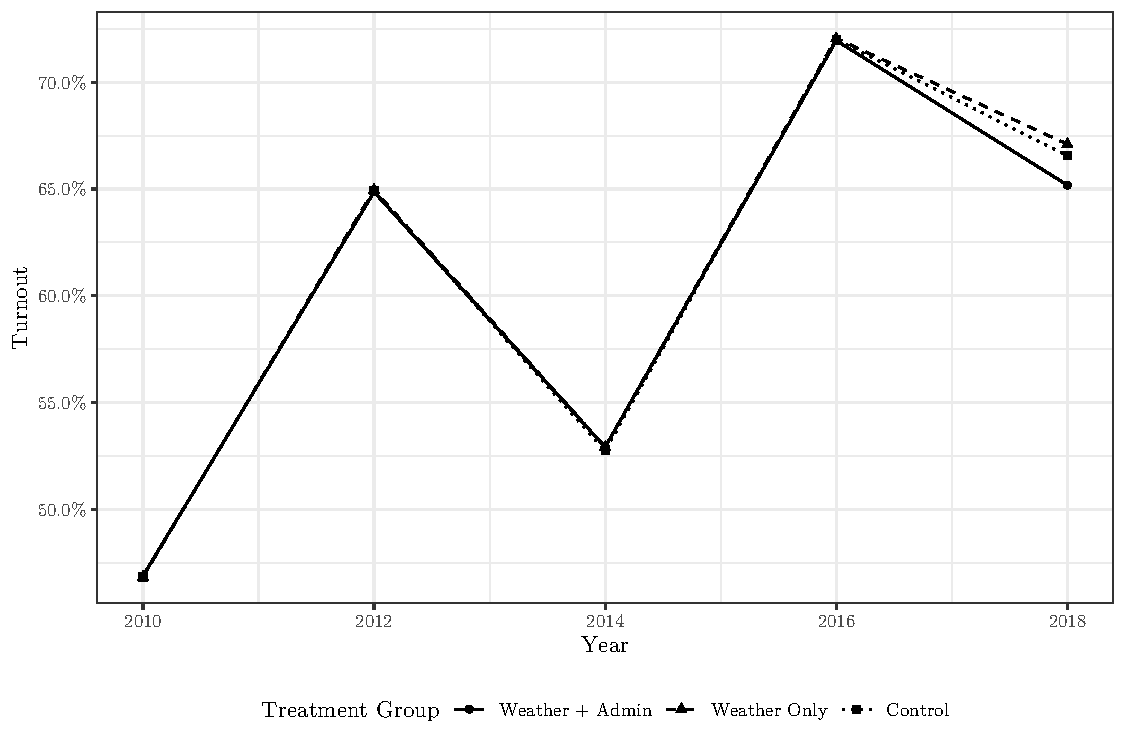
\includegraphics{hurricane_michael_files/figure-latex/tripd-to-chunk-1} 

}

\caption{\label{fig:trip-diff-plot}General Election Turnout for Treated, Primary Control, and Secondary Control Voters, 2010 -- 2018}\label{fig:tripd-to-chunk}
\end{figure}

Disentangling the administrative and individual effects of the storm requires the estimation of the triple-differences model. This model is estimated by Equation (1).

\begin{gather}
\label{eq:1}
v_{it}=\beta_0+\beta_1Panhandle_{i}+\beta_22018_{t}+\beta_3Panhandle_{i}\times 2018_{t} + \nonumber \\
\beta_4Treated_{i} + \beta_5Treated_{i}\times 2018_{t} + \\
\delta{Y}_{it} + \delta{Z}_{i} + \mathcal{E}_{it}. \nonumber
\end{gather}

Individual \emph{i}'s turnout (\emph{v}) in year \emph{t} is a function of the year and their location. In the equation, \emph{\(\beta\)\textsubscript{1}Panhandle\textsubscript{i}} measures the historical difference between voters in the panhandle and the rest of the state. \emph{\(\beta\)\textsubscript{2}2018\textsubscript{t}} measures the statewide change in turnout in 2018 from the baseline, while \emph{\(\beta\)\textsubscript{3}Panhandle\textsubscript{i} × 2018\textsubscript{t}} tests whether turnout changed differently in 2018 in the panhandle than it did elsewhere. \emph{\(\beta\)\textsubscript{3}Panhandle\textsubscript{i} × 2018\textsubscript{t}}, therefore, is our estimation of the individual-level, or weather related, effect of the hurricane. \emph{\(\beta\)\textsubscript{4}Treated\textsubscript{i}} measures the historical difference between treated and primary control voters, and \emph{\(\beta\)\textsubscript{5}Treated\textsubscript{i} × 2018\textsubscript{t}} tests whether the causal effect of the storm was different for treated voters than for their primary controls. This, then, is the estimated administrative effect of living in a county covered by the executive order. The matrix \emph{\(\delta\)Y\textsubscript{i}} includes the measures for relative rainfall and polling place closures interacted with treatment, panhandle, and 2018 dummies. The matrix \emph{\(\delta\)Z\textsubscript{i}} includes the covariates used in the matching procedure.

Table \ref{tab:trip-diff} presents the results of this model, again fit using an ordinary least squares specification. Model 1 does not include \emph{\(\delta\)Z\textsubscript{i}}, while the matrix is included in Models 2 and 3. Model 3 also includes estimates for congressional district competitiveness in 2018. Finally, in Model 4, we once again investigate whether the treatment effect was moderated by polling place closures and relative rainfall. While the models include the full matrix \emph{\(\delta\)Y\textsubscript{i}}, we display only rain and polling place closures' influence on the treatment effect in the table for the sake of legibility. Robust standard errors are clustered at the level of the original treated voter from which the primary and secondary controls arise.

\begin{singlespace}

\input{"../temp/triple_diff.tex"}
\end{singlespace}

The coefficients on \emph{Panhandle × 2018} and \emph{Treated × 2018} are of most substantive interest here. The coefficient on \emph{Panhandle × 2018} indicates that turnout for the primary control voters in 2018 was not statistically significantly different than the 2018 turnout of the secondary controls, Hurricane Michael notwithstanding. Given that these counties were not covered by the executive order because they were not in the direct path of the storm, this lack of a turnout effect is unsurprising.

There was, however, a negative treatment effect for voters just inside the treated counties. \emph{Treated × 2018} in models 1--3 indicates that, for voters just inside the treated counties, turnout was depressed relative to their primary controls by 1.9 percentage points. This 1.9 percentage point decrease in turnout for voters inside the treated counties is the administrative effect on turnout.

Model 4 once again demonstrates that these effects were moderated by polling place consolidation and the strength of the storm---with polling place consolidation having a far larger impact. In this set of treated voters, there is a negative relationship between polling place consolidation and relative rainfall. Treated voters in Bay County (where 6 of 44 polling places were open) saw rainfall 155\% of normal; in Gadsden and Liberty Counties where the expected number of polling places were open, by contrast, treated voters saw rainfall that was 213\% and 229\% of normal, respectively. Multiplying out the coefficients from model 4 in Table \ref{tab:trip-diff} results in an estimated administrative treatment effects ranging from -6.4 points in Bay County to +0.35 points in Gadsden. Once again, we see that county-level polling place consolidation had a far larger influence on turnout than the storm itself.

Importantly, the decomposed administrative- and individual- effects estimated in Table \ref{tab:trip-diff} are the average treatment effect on the treated voters (ATT). Nevertheless, the administrative effect of -1.9 percentage points is substantively quite large. Despite the efforts of Executive Order 18-283, the administrative costs imposed by Hurricane Michael meaningfully depressed turnout. As model 4 indicates, however, the executive order may have \emph{increased} turnout where counties were able to keep the bulk of their polling places open.

\hypertarget{shifting-vote-modes}{%
\section*{Shifting Vote Modes}\label{shifting-vote-modes}}
\addcontentsline{toc}{section}{Shifting Vote Modes}

Having established that turnout was substantially depressed in the treated counties and that a non-trivial amount of the depression arose from administrative costs, we turn to a new question: did the storm shift \emph{how} people cast their ballots? We know that Executive Order 18-283 loosened restrictions on early and mail balloting; we therefore expect that, relative to the rest of the state, a higher share of ballots in the treated counties cast their ballots in one of these ways.

We return to the matches produced earlier in this paper, where every voter in the treated counties was matched with five voters elsewhere in the state. Figure \ref{fig:vote-mode} demonstrates the share of registered voters that cast a ballot either at the polling place, early in person, or absentee in each general election from the past decade. In each case, the denominator is the number of registered voters in 2018.

\begin{figure}[h]

{\centering 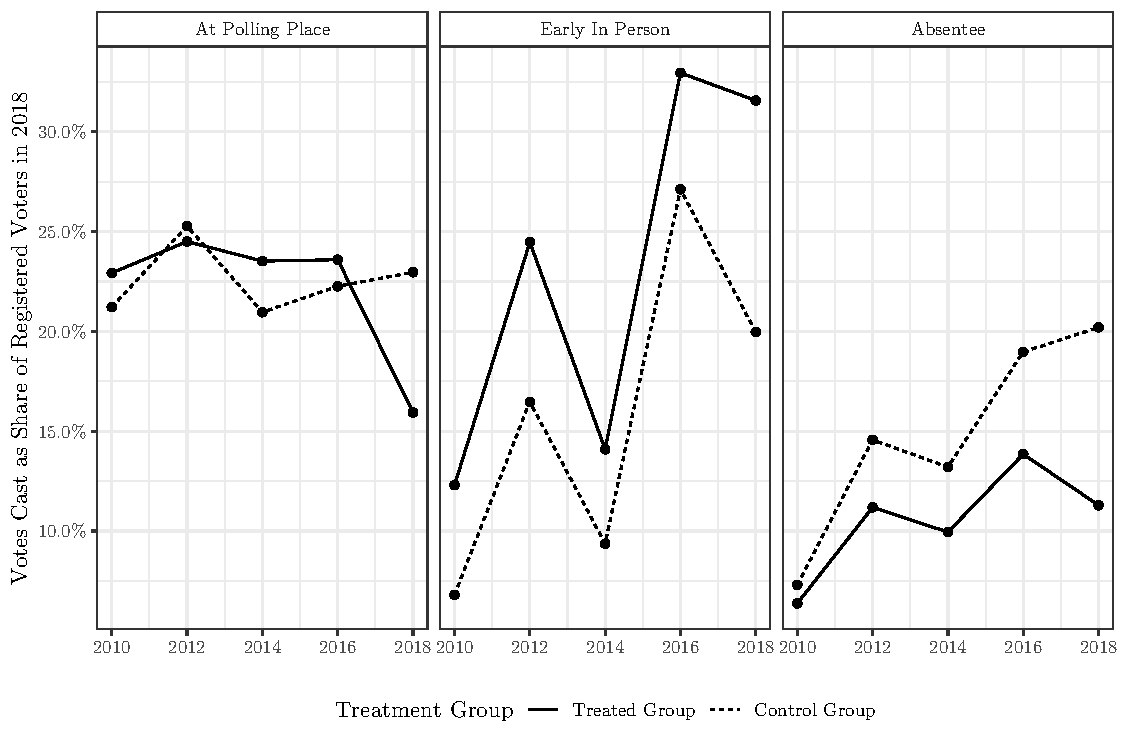
\includegraphics{hurricane_michael_files/figure-latex/vote-mode-chunk-1} 

}

\caption{\label{fig:vote-mode}Marginal Effect of Relocated Polling Place on Vote Mode}\label{fig:vote-mode-chunk}
\end{figure}

Figure \ref{fig:vote-mode} makes clear that the decline in turnout was a product of lower turnout on election day and via absentee voting. It seems, however, that early voting was actually higher in the treated counties due to Hurricane Michael.

To more directly estimate the effect of Hurricane Michael and the executive order on vote-mode, we measure how far each treated voter lived from the closest planned polling place and the polling place that actually opened on election day. Using a multinomial logistic regression, we test whether increasing the difference between this distance is related to vote-mode or abstention in 2018. In addition to the difference between expected and actual distance to the closest polling place, we include other covariates. We measure how far a voter lived from her closest \emph{planned} polling place, in case voters in more remote parts of the counties generally voted differently in 2018 than other voters. We include other covariates for individual characteristics such as race, age, and partisan affiliation. We also include dummies indicating how (or whether) each voter participated in the 2012 -- 2016 general elections.

Because the coefficients from the mulinomial logistic regression are difficult to interpret on their own, we include here the marginal effects plots from this model (the full regression table can be found in the Supplementary Information). Figure \ref{fig:marg-multi} presents the marginal effect of the change in distance to the nearest polling place on vote method while keeping all other covariates in the model at their means.

\begin{figure}[h]

{\centering 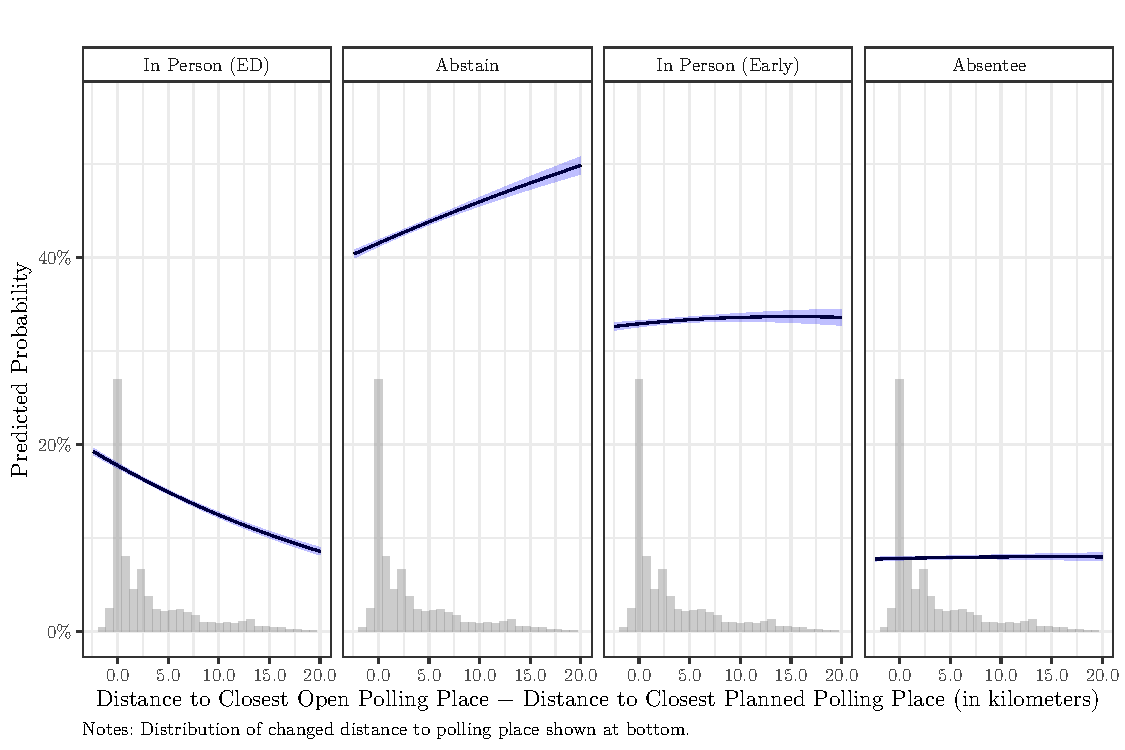
\includegraphics{hurricane_michael_files/figure-latex/marg-multi-1} 

}

\caption{\label{fig:marg-multi}Marginal Effect of Changed Distance to Polling Place on 2018 Vote Mode}\label{fig:marg-multi}
\end{figure}

Figure \ref{fig:marg-multi} indicates that, as voters suddenly had to travel further to the nearest polling place, they were substantially less likely to vote in person on election day (``In Person (ED)''). The bulk of these voters \emph{did not} shift to absentee voting or early in-person voting; rather, they were much more likely to abstain from casting a ballot at all. Thus, although administrators took steps to make early and mail voting easier, these efforts were not particularly effective.

\hypertarget{discussion-and-conclusion}{%
\section*{Discussion and Conclusion}\label{discussion-and-conclusion}}
\addcontentsline{toc}{section}{Discussion and Conclusion}

Election Day in the United States consistently falls near the end of hurricane season. Hurricane Michael made landfall on October 10, 2018, less than a month before the highest-turnout midterm election in a century. Hurricane Sandy struck New York and New Jersey just days before the midterm elections in 2012, wreaking immense havoc. Hurricane Matthew struck the Southeastern United States weeks before the 2016 presidential election, killing dozens and causing more than \$2.5 billion in damages. \protect\hyperlink{ref-Mann2006}{Mann and Emanuel} (\protect\hyperlink{ref-Mann2006}{2006}) and others have linked Atlantic hurricanes to climate change, indicating that these disruptions to election day activity are likely to increase in coming years. Understanding how storms of this nature impact turnout --- and whether states' responses are sufficient to recoup turnout --- is therefore vitally important, particularly in swing states such as Florida and North Carolina that are subject to severe coastal natural disasters.

As this paper demonstrates, Florida's response to Hurricane Michael was not particularly effective: although Governor Scott increased access to early and mail voting in eight counties, mail balloting use in these areas actually \emph{dropped} relative to the rest of the state (see Figure \ref{fig:vote-mode}). Despite the executive order, turnout dropped substantially for voters who suddenly were faced with long distances to the closest polling places. These voters did not move to vote-by-mail options in appreciable numbers.

This is disheartening. Not only did the executive order fail to combat the negative individual-level effects of the hurricane on turnout, it was also insufficient at mitigating the negative administrative effects of closed polling places. Clearly, loosening restrictions on where mail ballots could be sent and how they could be returned was not enough. Without the executive order, polling places would still have been moved because some had been destroyed, but the loosened restrictions on other modes would not have been accessible. Thus, the executive order likely reduced the administrative costs of voting. Nevertheless, these administrative effects remained quite large and were responsible for nearly half the depressive effect of the storm for voters living at the outer edges of the covered counties.

The data at hand cannot explain why the executive order was ineffective at neutralizing the administrative effects of the hurricane. The timing of the executive order, however, might shed some light. Although the hurricane made landfall on October 10, the executive order was not signed until more than a week later, on October 18 --- fewer than three weeks before the November 6 general election. This left little time for an effective public education campaign, perhaps limiting the number of voters who learned and took advantage of the changed rules. We found very few news articles detailing the changes and making the information easily available to voters (but see \protect\hyperlink{ref-WJHG2018}{\emph{WJHG - Panama City} 2018}; \protect\hyperlink{ref-Vasquez2018}{Vasquez 2018}; \protect\hyperlink{ref-McDonald2018}{McDonald 2018}; \protect\hyperlink{ref-Fineout2018}{Fineout 2018}), and what information did get published often listed only relocated polling places with no information about loosened mail voting restrictions (see, for instance, \protect\hyperlink{ref-gadsdentimes2018}{\emph{Gadsden Times} 2018}). It is possible, of course, that local televised news communicated the changes to viewers; however, based on our search of published information, that information would have been difficult to find for voters who missed the televised news. We found no evidence that the Florida Times-Union (the largest paper in Northern Florida) or the Tampa Bay Times (the largest paper in the state) published any articles detailing the changes brought about by the executive order.

Future research will no doubt leverage pre-existing administrative regimes to understand the sorts of voting environments least susceptible to disruption, like those following from the coronavirus in the context of the 2020 elections --- but such research will necessarily be backward looking. The experience of Hurricane Michael, on the other hand, gives us important insight about how an emergency that closes polling places will structure turnout. Our research on Executive Order 18-283 makes clear that loosened restrictions on mail voting alone cannot combat the negative turnout effects of shuttered polling places.

\sout{The novel coronavirus will perhaps lower turnout even if election administrators respond perfectly. Voting might be low on a list of priorities for individuals who are caring for ailing loved ones, grieving, or dealing with economic crises. Nevertheless, COVID-19 will also pose administrative hurdles to voting: consolidated or relocated polling places, reliance on a vote-by-mail system unfamiliar to many voters, or longer wait times as the number of voters allowed into a polling place at once might all reduce turnout. As administrators consider easing vote-by-mail restrictions, they must look to the case of Florida in 2018. More must be done than simply change the rules; otherwise, the administrative effects of COVID-19 will magnify the individual effects of this public health crisis on voter turnout.}

\newpage

\hypertarget{references}{%
\section*{References}\label{references}}
\addcontentsline{toc}{section}{References}

\hypertarget{refs}{}
\begin{CSLReferences}{1}{0}
\leavevmode\hypertarget{ref-Abadie2020}{}%
Abadie, Alberto, and Jann Spiess. 2020. {``Robust {Post}-{Matching Inference}.''} \emph{Journal of the American Statistical Association} 0 (0): 1--13. \url{https://doi.org/10.1080/01621459.2020.1840383}.

\leavevmode\hypertarget{ref-Barber2020}{}%
Barber, Michael, and John Holbein. 2020. {``The Participatory and Partisan Impacts of Mandatory Vote-by-Mail.''} \emph{Science Advances} 6 (35). \url{https://doi.org/10.1126/sciadv.abc7685}.

\leavevmode\hypertarget{ref-Bergman2015}{}%
Bergman, Elizabeth. 2015. {``Voting Only by Mail Can Decrease Turnout. {Or} Increase It. {Wait}, What?''} \emph{Washington Post}, December 21, 2015. \url{https://www.washingtonpost.com/news/monkey-cage/wp/2015/12/21/voting-only-by-mail-can-decrease-or-increase-turnout-wait-what/}.

\leavevmode\hypertarget{ref-Bergman2011}{}%
Bergman, Elizabeth, and Philip Yates. 2011. {``Changing {Election Methods}: {How Does Mandated Vote}-by-{Mail Affect Individual Registrants}?''} \emph{Election Law Journal} 10 (2): 115--27.

\leavevmode\hypertarget{ref-Brady2011}{}%
Brady, Henry, and John McNulty. 2011. {``Turning Out to Vote: {The Costs} of {Finding} and {Getting} to the {Polling Place}.''} \emph{American Political Science Review} 105 (1): 115--34.

\leavevmode\hypertarget{ref-Burden2014}{}%
Burden, Barry C., David T. Canon, Kenneth R. Mayer, and Donald P. Moynihan. 2014. {``Election {Laws}, {Mobilization}, and {Turnout}: {The Unanticipated Consequences} of {Election Reform}.''} \emph{American Journal of Political Science} 58 (1): 95--109. \url{https://doi.org/10.1111/ajps.12063}.

\leavevmode\hypertarget{ref-Cantoni2020}{}%
Cantoni, Enrico. 2020. {``A {Precinct Too Far}: {Turnout} and {Voting Costs}.''} \emph{American Economic Journal: Applied Economics} 12 (1): 61--85.

\leavevmode\hypertarget{ref-Cooperman2017}{}%
Cooperman, Alicia. 2017. {``Randomization {Inference} with {Rainfall Data}: {Using Historical Weather Patterns} for {Variance Estimation}.''} \emph{Political Analysis} 25 (3): 277--88.

\leavevmode\hypertarget{ref-Debbage2014}{}%
Debbage, Neil, Nick Gonsalves, J. Marshall Shepherd, and John Knox. 2014. {``Superstorm {Sandy} and {Voter Vulnerability} in the 2012 {US Presidential Election}: {A Case Study} of {New Jersey} and {Connecticut}.''} \emph{Environmental Hazards} 13: 181--99.

\leavevmode\hypertarget{ref-Dyck2005}{}%
Dyck, Joshua, and James Gimpel. 2005. {``Distance, {Turnout}, and the {Convenience} of {Voting}.''} \emph{Social Science Quarterly} 86 (3): 531--48.

\leavevmode\hypertarget{ref-Elul2017}{}%
Elul, Gabrielle, Sean Freeder, and Jacob Grumbach. 2017. {``The {Effect} of {Mandatory Mail Ballot Elections} in {California}.''} \emph{Election Law Journal} 16 (3): 397--415.

\leavevmode\hypertarget{ref-Fineout2018}{}%
Fineout, Gary. 2018. {``Florida to Bend Voting Rules in Counties Hit by Hurricane.''} \emph{Northwest Florida Daily News}, October 18, 2018. \url{https://www.nwfdailynews.com/news/20181018/florida-to-bend-voting-rules-in-counties-hit-by-hurricane}.

\leavevmode\hypertarget{ref-Fitzgerald2005}{}%
Fitzgerald, Mary. 2005. {``Greater {Convenience But Not Greater Turnout}: {The Impact} of {Alternative Voting Methods} on {Electoral Participation} in the {United States}.''} \emph{American Politics Research} 33 (6): 842--67. \url{https://doi.org/10.1177/1532673X04274066}.

\leavevmode\hypertarget{ref-Fraga2010}{}%
Fraga, Bernard, and Eitan Hersh. 2010. {``Voting {Costs} and {Voter Turnout} in {Competitive Elections}.''} \emph{Quarterly Journal of Political Science} 5: 339--56. https://doi.org/\url{http://dx.doi.org/10.1561/100.00010093_supp}.

\leavevmode\hypertarget{ref-Fujiwara2016}{}%
Fujiwara, Thomas, Kyle Meng, and Tom Vogl. 2016. {``Habit {Formation} in {Voting}: {Evidence} from {Rainy Elections}.''} \emph{American Economic Journal: Applied Economics} 8 (4): 160--88.

\leavevmode\hypertarget{ref-gadsdentimes2018}{}%
\emph{Gadsden Times}. 2018. {``Changes in Polling Places at Three Locations,''} October 30, 2018. \url{https://www.gadsdentimes.com/news/20181030/changes-in-polling-places-at-three-locations}.

\leavevmode\hypertarget{ref-Gatrell2002}{}%
Gatrell, Jay, and Gregory Bierly. 2002. {``Weather and {Voter Turnout}: {Kentucky Primary} and {General Elections}, 1990-2000.''} \emph{Southeastern Geographer} 42 (1): 114--34.

\leavevmode\hypertarget{ref-Gerber2013}{}%
Gerber, Alan, Gregory Huber, and Seth Hill. 2013. {``Identifying the {Effect} of {All}-{Mail Elections} on {Turnout}: {Staggered Reform} in the {Evergreen State}.''} \emph{Political Science Research and Methods} 1 (1): 91--116.

\leavevmode\hypertarget{ref-Gimpel2003}{}%
Gimpel, James, and Jason Schuknecht. 2003. {``Political {Participation} and the {Accessibility} of the {Ballot Box}.''} \emph{Political Geography} 22: 471--88.

\leavevmode\hypertarget{ref-Gomez2007}{}%
Gomez, Brad, Thomas Hansford, and George Krause. 2007. {``The {Republicans Should Pray} for {Rain}: {Weather}, {Turnout}, and {Voting} in {U}.{S}. {Presidential Elections}.''} \emph{Journal of Politics} 69: 649--63.

\leavevmode\hypertarget{ref-Gronke2008}{}%
Gronke, Paul, Eva Galanes-Rosenbaum, Peter A. Miller, and Daniel Toffey. 2008. {``Convenience {Voting}.''} \emph{Annual Review of Political Science} 11 (1): 437--55. \url{https://doi.org/10.1146/annurev.polisci.11.053006.190912}.

\leavevmode\hypertarget{ref-Gronke2012}{}%
Gronke, Paul, and Peter Miller. 2012. {``Voting by {Mail} and {Turnout} in {Oregon}: {Revisiting Southwell} and {Burchett}.''} \emph{American Politics Research} 40 (6): 976--97. \url{https://doi.org/10.1177/1532673X12457809}.

\leavevmode\hypertarget{ref-Hansford2010}{}%
Hansford, Thomas, and Brad Gomez. 2010. {``Estimating the {Electoral Effects} of {Voter Turnout}.''} \emph{American Political Science Review} 104: 268--88.

\leavevmode\hypertarget{ref-Haspel2005}{}%
Haspel, Moshe, and H. Gibbs Knotts. 2005. {``Location, {Location}, {Location}: {Precinct Placement} and the {Costs} of {Voting}.''} \emph{Journal of Politics} 67 (2): 560--73.

\leavevmode\hypertarget{ref-Henrickson2019}{}%
Henrickson, Kevin E., and Erica H. Johnson. 2019. {``Increasing {Voter Participation} by {Altering} the {Costs} and {Stakes} of {Voting}*.''} \emph{Social Science Quarterly} 100 (3): 869--84. \url{https://doi.org/10.1111/ssqu.12583}.

\leavevmode\hypertarget{ref-James2020}{}%
James, Toby, and Sead Alihodzic. 2020. {``When {Is It Democratic} to {Postpone} an {Election}? {Elections During Natural Disasters}, {COVID}-19, and {Emergency Situations}.''} \emph{Election Law Journal} 19 (3): 344--62. \url{https://doi.org/10.1089/elj.2020.0642}.

\leavevmode\hypertarget{ref-Kaplan2020}{}%
Kaplan, Ethan, and Haishan Yuan. 2020. {``Early {Voting Laws}, {Voter Turnout}, and {Partisan Vote Composition}: {Evidence} from {Ohio}.''} \emph{American Economic Journal: Applied Economics} 12 (1): 32--60.

\leavevmode\hypertarget{ref-Keele2015a}{}%
Keele, Luke, Rocío Titiunik, and José R. Zubizarreta. 2015. {``Enhancing a Geographic Regression Discontinuity Design Through Matching to Estimate the Effect of Ballot Initiatives on Voter Turnout.''} \emph{Journal of the Royal Statistical Society: Series A (Statistics in Society)} 178 (1): 223--39. \url{https://doi.org/10.1111/rssa.12056}.

\leavevmode\hypertarget{ref-Kitamura2020}{}%
Kitamura, Shuhei, and Tetsuya Matsubayashi. 2020. {``Dynamic {Voting}.''}

\leavevmode\hypertarget{ref-Knack1994}{}%
Knack, Stephen. 1994. {``Does {Rain Help} the {Republicans}? {Theory} and {Evidence} on {Turnout} and the {Vote}.''} \emph{Public Choice} 79: 189--204.

\leavevmode\hypertarget{ref-Kousser2007}{}%
Kousser, Thad, and Megan Mullin. 2007. {``Does {Voting} by {Mail Increase Participation}? {Using Matching} to {Analyze} a {Natural Experiment}.''} \emph{Political Analysis} 15 (4): 428--45. \url{http://www.jstor.org/stable/25791905}.

\leavevmode\hypertarget{ref-Kropf2012}{}%
Kropf, Martha, and David Kimball. 2012. \emph{Helping {America Vote}: {The Limits} of {Election Reform}}. {New York}: {Routledge}.

\leavevmode\hypertarget{ref-Larocca2011}{}%
Larocca, Roger, and John S. Klemanski. 2011. {``U.{S}. {State Election Reform} and {Turnout} in {Presidential Elections}.''} \emph{State Politics \& Policy Quarterly} 11 (1): 76--101. \url{https://doi.org/10.1177/1532440010387401}.

\leavevmode\hypertarget{ref-Lasala-Blanco2017}{}%
Lasala-Blanco, Narayani, Robert Shapiro, and Viviana Rivera-Burgos. 2017. {``Turnout and {Weather Disruptions}: {Survey Evidence} from the 2012 {Presidential Elections} in the {Aftermath} of {Hurricane Sandy}.''} \emph{Electoral Studies} 45: 141--52.

\leavevmode\hypertarget{ref-Leighley2014}{}%
Leighley, Jan, and Jonathan Nagler. 2014. \emph{Who {Votes Now}? {Demographics}, {Issues}, {Inequality}, and {Turnout} in the {United States}}. {Princeton}: {Princeton University Press}.

\leavevmode\hypertarget{ref-Mann2006}{}%
Mann, Michael E., and Kerry A. Emanuel. 2006. {``Atlantic Hurricane Trends Linked to Climate Change.''} \emph{Eos, Transactions American Geophysical Union} 87 (24): 233--41. \url{https://doi.org/10.1029/2006EO240001}.

\leavevmode\hypertarget{ref-McDonald2018}{}%
McDonald, Zack. 2018. {``Bay Voters Getting 5 'Mega Voting' Sites.''} \emph{Panama City News Herald}, October 23, 2018. \url{https://www.newsherald.com/news/20181023/bay-voters-getting-5-mega-voting-sites}.

\leavevmode\hypertarget{ref-McNulty2009}{}%
McNulty, John, Conor Dowling, and Margaret Ariotti. 2009. {``Driving {Saints} to {Sin}: {How Increasing} the {Difficulty} of {Voting Dissuades Even} the {Most Motivated Voters}.''} \emph{Political Analysis} 17 (4): 435--55.

\leavevmode\hypertarget{ref-Merrifield1993}{}%
Merrifield, John. 1993. {``The {Institutional} and {Political Factors} That {Influence Voter Turnout}.''} \emph{Public Choice} 77: 657--67.

\leavevmode\hypertarget{ref-Nyhan2017}{}%
Nyhan, Brendan, Christopher Skovron, and Rocío Titiunik. 2017. {``Differential {Registration Bias} in {Voter File Data}: {A Sensitivity Analysis Approach}.''} \emph{American Journal of Political Science} 61 (3): 744--60. \url{https://doi.org/10.1111/ajps.12288}.

\leavevmode\hypertarget{ref-Parks2018}{}%
Parks, Miles. 2018. {``After {Hurricane Michael}, {Voting} '{Is The Last Thing On Their Minds}'.''} \emph{NPR.org}, October 25, 2018. \url{https://www.npr.org/2018/10/25/659819848/after-hurricane-michael-voting-is-the-last-thing-on-their-minds}.

\leavevmode\hypertarget{ref-Persson2014}{}%
Persson, Mikael, Anders Sundell, and Richard Öhrvall. 2014. {``Does {Election Day Weather Affect Voter Turnout}? {Evidence} from {Swedish Elections}.''} \emph{Electoral Studies} 33: 335--42.

\leavevmode\hypertarget{ref-Rallings2003}{}%
Rallings, Colin, Michael Thrasher, and Roman Borisyuk. 2003. {``Seasonal {Factors}, Voter Fatigue, and the Costs of Voting.''} \emph{Electoral Studies} 22: 65--79.

\leavevmode\hypertarget{ref-Ricardson1996}{}%
Ricardson, Lilliard, and Grant Neeley. 1996. {``The {Impact} of {Early Voting} on {Turnout}: {The} 1994 {Elections} in {Tennessee}.''} \emph{State \& Local Government Review} 28 (3): 173--79.

\leavevmode\hypertarget{ref-Sekhon2009}{}%
Sekhon, Jasjeet. 2009. {``Opiates for the {Matches}: {Matching Methods} for {Causal Inference}.''} \emph{Annual Review of Political Science} 12: 487--508.

\leavevmode\hypertarget{ref-Sekhon2011}{}%
---------. 2011. {``Multivariate and {Propensity Score Matching Software} with {Automated Balance Optimization}: {The Matching} Package for {R}.''} \emph{Journal of Statistical Software} 42 (1): 1--52. \url{https://doi.org/10.18637/jss.v042.i07}.

\leavevmode\hypertarget{ref-Shachar1999}{}%
Shachar, Ron, and Barry Nalebuff. 1999. {``Follow the {Leader}: {Theory} and {Evidence} on {Political Participation}.''} \emph{American Economic Review} 89 (3): 525--47.

\leavevmode\hypertarget{ref-Sinclair2011}{}%
Sinclair, Betsy, Thad E. Hall, and R. Michael Alvarez. 2011. {``Flooding the {Vote}: {Hurricane Katrina} and {Voter Participation} in {New Orleans}.''} \emph{American Politics Research} 39 (5): 921--57. \url{https://doi.org/10.1177/1532673X10386709}.

\leavevmode\hypertarget{ref-Stein2015}{}%
Stein, Robert. 2015. {``Election {Administration During National Disasters} and {Emergencies}: {Hurricane Sandy} and the 2012 {Election}.''} \emph{Election Law Journal} 14: 66--73.

\leavevmode\hypertarget{ref-Vasquez2018}{}%
Vasquez, Savannah. 2018. {``{HURRICANE MICHAEL}: {How} to Vote in {Gulf County}.''} \emph{The Star}, October 18, 2018. \url{https://www.starfl.com/news/20181018/hurricane-michael-how-to-vote-in-gulf-county}.

\leavevmode\hypertarget{ref-Walker2019}{}%
Walker, Hannah L., Michael C. Herron, and Daniel A. Smith. 2019. {``Early {Voting Changes} and {Voter Turnout}: {North Carolina} in the 2016 {General Election}.''} \emph{Political Behavior} 41 (4): 841--69. \url{https://doi.org/10.1007/s11109-018-9473-5}.

\leavevmode\hypertarget{ref-WJHG2018}{}%
\emph{WJHG - Panama City}. 2018. {``Bay {County Hurricane Michael Recovery Information},''} October 31, 2018. \url{https://www.wjhg.com/content/news/Bay-County–498037961.html}.

\end{CSLReferences}

\end{document}
